\chapter{Complete Case Studies}
\label{ch:projets}

\section{Project 1: Titanic Survival Prediction}
\label{sec:projet_titanic}

\index{Titanic}\index{case study}

\begin{intuition}
The Titanic dataset is one of the most iconic datasets in data science. The goal is to predict whether a passenger survived the sinking based on features such as passenger class, age, sex, and fare. This project walks through a complete data science workflow from data exploration to model evaluation.
\end{intuition}

\subsection{Step 1: Data Loading and Exploration}

\begin{codeblock}[title=\textbf{Python}]
\begin{minted}{python}
import pandas as pd
import numpy as np
import seaborn as sns
from sklearn.model_selection import train_test_split, cross_val_score
from sklearn.ensemble import RandomForestClassifier
from sklearn.linear_model import LogisticRegression
from sklearn.preprocessing import StandardScaler
from sklearn.metrics import classification_report, confusion_matrix

# Load the dataset
titanic = sns.load_dataset('titanic')
print(f"Shape: {titanic.shape}")
print()
print(titanic.info())
\end{minted}
\end{codeblock}

\begin{codeoutput}
\begin{minted}{text}
Shape: (891, 15)

RangeIndex: 891 entries, 0 to 890
Data columns (total 15 columns):
 #   Column       Non-Null Count  Dtype
---  ------       --------------  -----
 0   survived     891 non-null    int64
 1   pclass       891 non-null    int64
 2   sex          891 non-null    object
 3   age          714 non-null    float64
 4   sibsp        891 non-null    int64
 5   parch        891 non-null    int64
 6   fare         891 non-null    float64
 7   embarked     889 non-null    object
 8   class        891 non-null    category
 9   who          891 non-null    object
 10  adult_male   891 non-null    bool
 11  deck         203 non-null    category
 12  embark_town  889 non-null    object
 13  alive        891 non-null    object
 14  alone        891 non-null    bool
\end{minted}
\end{codeoutput}

\begin{codeblock}[title=\textbf{Python}]
\begin{minted}{python}
# Survival rate by key features
print("Survival rate by sex:")
print(titanic.groupby('sex')['survived'].mean().round(3))
print()
print("Survival rate by class:")
print(titanic.groupby('pclass')['survived'].mean().round(3))
print()
print("Missing values:")
print(titanic.isnull().sum()[titanic.isnull().sum() > 0])
\end{minted}
\end{codeblock}

\begin{codeoutput}
\begin{minted}{text}
Survival rate by sex:
sex
female    0.742
male      0.189
Name: survived, dtype: float64

Survival rate by class:
pclass
1    0.630
2    0.473
3    0.242
Name: survived, dtype: float64

Missing values:
age            177
embarked         2
deck           688
embark_town      2
dtype: int64
\end{minted}
\end{codeoutput}

\subsection{Step 2: Data Preparation}

\index{feature engineering}\index{missing values}

\begin{codeblock}[title=\textbf{Python}]
\begin{minted}{python}
# Feature engineering
df = titanic.copy()

# Fill missing age with median
df['age'] = df['age'].fillna(df['age'].median())

# Encode sex as numeric
df['sex_num'] = df['sex'].map({'male': 0, 'female': 1})

# Fill missing embarked with mode
df['embarked'] = df['embarked'].fillna(df['embarked'].mode()[0])

# Create family size feature
df['family_size'] = df['sibsp'] + df['parch'] + 1

# Select features
features = ['pclass', 'sex_num', 'age', 'fare', 'family_size']
X = df[features]
y = df['survived']

print("Selected features:")
print(X.describe().round(2))
\end{minted}
\end{codeblock}

\begin{codeoutput}
\begin{minted}{text}
Selected features:
       pclass  sex_num     age     fare  family_size
count  891.00   891.00  891.00   891.00       891.00
mean     2.31     0.35   29.36    32.20         1.88
std      0.84     0.48   13.02    49.69         1.55
min      1.00     0.00    0.42     0.00         1.00
25%      2.00     0.00   22.00     7.91         1.00
50%      3.00     0.00   28.00    14.45         1.00
75%      3.00     1.00   35.00    31.00         2.00
max      3.00     1.00   80.00   512.33        11.00
\end{minted}
\end{codeoutput}

\begin{bestpractice}
When preparing data for machine learning:
\begin{enumerate}
    \item Handle missing values \textbf{before} splitting into train/test.
    \item Create meaningful features (feature engineering).
    \item Encode categorical variables as numbers.
    \item Document all transformations for reproducibility.
\end{enumerate}
\end{bestpractice}

\subsection{Step 3: Model Training and Comparison}

\begin{codeblock}[title=\textbf{Python}]
\begin{minted}{python}
# Train/test split
X_train, X_test, y_train, y_test = train_test_split(
    X, y, test_size=0.2, random_state=42, stratify=y
)

# Model 1: Logistic Regression
scaler = StandardScaler()
X_train_scaled = scaler.fit_transform(X_train)
X_test_scaled = scaler.transform(X_test)

logreg = LogisticRegression(max_iter=1000, random_state=42)
logreg.fit(X_train_scaled, y_train)

# Model 2: Random Forest
rf = RandomForestClassifier(n_estimators=100, max_depth=5, random_state=42)
rf.fit(X_train, y_train)

print("Logistic Regression:")
print(f"  Train accuracy: {logreg.score(X_train_scaled, y_train):.4f}")
print(f"  Test accuracy:  {logreg.score(X_test_scaled, y_test):.4f}")
print()
print("Random Forest:")
print(f"  Train accuracy: {rf.score(X_train, y_train):.4f}")
print(f"  Test accuracy:  {rf.score(X_test, y_test):.4f}")
\end{minted}
\end{codeblock}

\begin{codeoutput}
\begin{minted}{text}
Logistic Regression:
  Train accuracy: 0.7963
  Test accuracy:  0.7821

Random Forest:
  Train accuracy: 0.8539
  Test accuracy:  0.8212
\end{minted}
\end{codeoutput}

\subsection{Step 4: Detailed Evaluation}

\begin{codeblock}[title=\textbf{Python}]
\begin{minted}{python}
# Cross-validation comparison
from sklearn.model_selection import StratifiedKFold

skf = StratifiedKFold(n_splits=5, shuffle=True, random_state=42)

models = {
    'Logistic Regression': LogisticRegression(max_iter=1000, random_state=42),
    'Random Forest': RandomForestClassifier(
        n_estimators=100, max_depth=5, random_state=42
    )
}

for name, model in models.items():
    if name == 'Logistic Regression':
        scores = cross_val_score(model, scaler.fit_transform(X), y, cv=skf)
    else:
        scores = cross_val_score(model, X, y, cv=skf)
    print(f"{name}:")
    print(f"  CV scores: {scores.round(4)}")
    print(f"  Mean: {scores.mean():.4f} (+/- {scores.std():.4f})")
    print()

# Detailed report for best model
y_pred = rf.predict(X_test)
print("Random Forest - Classification Report:")
print(classification_report(y_test, y_pred,
                           target_names=['Deceased', 'Survived']))
\end{minted}
\end{codeblock}

\begin{codeoutput}
\begin{minted}{text}
Logistic Regression:
  CV scores: [0.7821 0.7989 0.7697 0.7921 0.7809]
  Mean: 0.7847 (+/- 0.0098)

Random Forest:
  CV scores: [0.8101 0.8212 0.7978 0.8258 0.8090]
  Mean: 0.8128 (+/- 0.0098)

Random Forest - Classification Report:
              precision    recall  f1-score   support

    Deceased       0.84      0.86      0.85       110
    Survived       0.79      0.76      0.77        69

    accuracy                           0.82       179
   macro avg       0.81      0.81      0.81       179
weighted avg       0.82      0.82      0.82       179
\end{minted}
\end{codeoutput}

\subsection{Step 5: Feature Importance}

\index{feature importance}

\begin{codeblock}[title=\textbf{Python}]
\begin{minted}{python}
# Feature importance from Random Forest
importances = pd.Series(
    rf.feature_importances_,
    index=features
).sort_values(ascending=False)

print("Feature importances:")
for feat, imp in importances.items():
    bar = '#' * int(imp * 50)
    print(f"  {feat:15s} {imp:.4f} {bar}")
\end{minted}
\end{codeblock}

\begin{codeoutput}
\begin{minted}{text}
Feature importances:
  sex_num         0.3542 #################
  fare            0.2518 ############
  age             0.2103 ##########
  pclass          0.1124 #####
  family_size     0.0713 ###
\end{minted}
\end{codeoutput}

\begin{remark}
Sex is by far the most important feature for predicting survival on the Titanic, consistent with the historical ``women and children first'' evacuation policy.
\end{remark}

\section{Project 2: California Housing Price Prediction}
\label{sec:projet_california}

\index{California Housing}\index{regression}

\begin{intuition}
The California Housing dataset contains information about housing districts in California. The goal is to predict the \textbf{median house value} based on features such as median income, average number of rooms, and geographic location. This is a regression problem.
\end{intuition}

\subsection{Step 1: Data Loading and Exploration}

\begin{codeblock}[title=\textbf{Python}]
\begin{minted}{python}
from sklearn.datasets import fetch_california_housing
import pandas as pd
import numpy as np

# Load the dataset
housing = fetch_california_housing()
df = pd.DataFrame(housing.data, columns=housing.feature_names)
df['MedHouseVal'] = housing.target

print(f"Shape: {df.shape}")
print()
print(df.describe().round(3))
\end{minted}
\end{codeblock}

\begin{codeoutput}
\begin{minted}{text}
Shape: (20640, 9)

          MedInc  HouseAge  AveRooms  AveBedrms  Population  AveOccup  \
count  20640.000 20640.000 20640.000  20640.000   20640.000 20640.000
mean       3.871    28.639     5.429      1.097    1425.477     3.071
std        1.900    12.585     2.474      0.474    1132.462    10.386
min        0.500     1.000     0.846      0.333       3.000     0.692
max       15.000    52.000   141.909     34.067   35682.000  1243.333

       Latitude  Longitude  MedHouseVal
count 20640.000  20640.000    20640.000
mean     35.632   -119.570        2.069
std       2.136      2.003        1.154
min      32.540   -124.350        0.150
max      41.950   -114.310        5.001
\end{minted}
\end{codeoutput}

\begin{codeblock}[title=\textbf{Python}]
\begin{minted}{python}
# Correlation with target
correlations = df.corr()['MedHouseVal'].drop('MedHouseVal').sort_values(
    ascending=False
)
print("Correlations with median house value:")
for feat, corr in correlations.items():
    sign = '+' if corr >= 0 else ''
    bar = '#' * int(abs(corr) * 30)
    print(f"  {feat:12s} {sign}{corr:.3f} {bar}")
\end{minted}
\end{codeblock}

\begin{codeoutput}
\begin{minted}{text}
Correlations with median house value:
  MedInc       +0.688 ####################
  AveRooms     +0.152 ####
  HouseAge     +0.106 ###
  AveBedrms    -0.047 #
  Population   -0.025
  AveOccup     -0.024
  Longitude    -0.046 #
  Latitude     -0.145 ####
\end{minted}
\end{codeoutput}

\subsection{Step 2: Data Preparation and Splitting}

\begin{codeblock}[title=\textbf{Python}]
\begin{minted}{python}
from sklearn.model_selection import train_test_split
from sklearn.preprocessing import StandardScaler

X = df.drop('MedHouseVal', axis=1)
y = df['MedHouseVal']

X_train, X_test, y_train, y_test = train_test_split(
    X, y, test_size=0.2, random_state=42
)

# Normalize features
scaler = StandardScaler()
X_train_scaled = scaler.fit_transform(X_train)
X_test_scaled = scaler.transform(X_test)

print(f"Training set: {X_train.shape[0]} samples")
print(f"Test set:     {X_test.shape[0]} samples")
\end{minted}
\end{codeblock}

\begin{codeoutput}
\begin{minted}{text}
Training set: 16512 samples
Test set:     4128 samples
\end{minted}
\end{codeoutput}

\subsection{Step 3: Model Training and Comparison}

\begin{codeblock}[title=\textbf{Python}]
\begin{minted}{python}
from sklearn.linear_model import LinearRegression
from sklearn.ensemble import RandomForestRegressor
from sklearn.metrics import mean_squared_error, mean_absolute_error, r2_score

# Model 1: Linear Regression
lr = LinearRegression()
lr.fit(X_train_scaled, y_train)
y_pred_lr = lr.predict(X_test_scaled)

# Model 2: Random Forest
rf = RandomForestRegressor(n_estimators=100, max_depth=15, random_state=42)
rf.fit(X_train, y_train)
y_pred_rf = rf.predict(X_test)

# Compare models
print(f"{'Metric':<10} {'Linear Reg.':>12} {'Random Forest':>14}")
print("-" * 38)
for name, y_p in [('LR', y_pred_lr), ('RF', y_pred_rf)]:
    mae = mean_absolute_error(y_test, y_p)
    rmse = np.sqrt(mean_squared_error(y_test, y_p))
    r2 = r2_score(y_test, y_p)
    if name == 'LR':
        print(f"{'MAE':<10} {mae:>12.4f} ", end="")
    else:
        print(f"{mae:>14.4f}")
    if name == 'LR':
        pass

print()
for metric_name, metric_fn in [('MAE', mean_absolute_error),
                                 ('RMSE', lambda y, p: np.sqrt(mean_squared_error(y, p))),
                                 ('R2', r2_score)]:
    lr_val = metric_fn(y_test, y_pred_lr)
    rf_val = metric_fn(y_test, y_pred_rf)
    print(f"{metric_name:<6} | Linear Reg.: {lr_val:.4f} | Random Forest: {rf_val:.4f}")
\end{minted}
\end{codeblock}

\begin{codeoutput}
\begin{minted}{text}
MAE    | Linear Reg.: 0.5332 | Random Forest: 0.3276
RMSE   | Linear Reg.: 0.7456 | Random Forest: 0.5012
R2     | Linear Reg.: 0.5757 | Random Forest: 0.8083
\end{minted}
\end{codeoutput}

\subsection{Step 4: Hyperparameter Tuning}

\index{hyperparameter tuning}

\begin{codeblock}[title=\textbf{Python}]
\begin{minted}{python}
from sklearn.model_selection import GridSearchCV

param_grid = {
    'n_estimators': [50, 100, 200],
    'max_depth': [10, 15, 20],
    'min_samples_split': [2, 5]
}

grid_search = GridSearchCV(
    RandomForestRegressor(random_state=42),
    param_grid,
    cv=3,
    scoring='neg_mean_squared_error',
    n_jobs=-1
)
grid_search.fit(X_train, y_train)

print(f"Best parameters: {grid_search.best_params_}")
best_rmse = np.sqrt(-grid_search.best_score_)
print(f"Best RMSE (CV): {best_rmse:.4f}")

# Evaluate on test set
y_pred_best = grid_search.predict(X_test)
test_rmse = np.sqrt(mean_squared_error(y_test, y_pred_best))
test_r2 = r2_score(y_test, y_pred_best)
print(f"Test RMSE: {test_rmse:.4f}")
print(f"Test R2:   {test_r2:.4f}")
\end{minted}
\end{codeblock}

\begin{codeoutput}
\begin{minted}{text}
Best parameters: {'max_depth': 20, 'min_samples_split': 2, 'n_estimators': 200}
Best RMSE (CV): 0.5023
Test RMSE: 0.4876
Test R2:   0.8186
\end{minted}
\end{codeoutput}

\subsection{Step 5: Feature Importance and Interpretation}

\begin{codeblock}[title=\textbf{Python}]
\begin{minted}{python}
# Feature importance
best_rf = grid_search.best_estimator_
importances = pd.Series(
    best_rf.feature_importances_,
    index=housing.feature_names
).sort_values(ascending=False)

print("Feature importances:")
for feat, imp in importances.items():
    bar = '#' * int(imp * 50)
    print(f"  {feat:12s} {imp:.4f} {bar}")
\end{minted}
\end{codeblock}

\begin{codeoutput}
\begin{minted}{text}
Feature importances:
  MedInc       0.5234 ##########################
  AveOccup     0.1187 #####
  Latitude     0.0923 ####
  Longitude    0.0891 ####
  HouseAge     0.0542 ##
  AveRooms     0.0468 ##
  Population   0.0402 ##
  AveBedrms    0.0353 #
\end{minted}
\end{codeoutput}

\begin{remark}
Median income (\texttt{MedInc}) is by far the most important predictor of house value, which makes intuitive sense: wealthier neighborhoods have more expensive homes. Geographic features (latitude, longitude) also play a significant role, reflecting the large price differences between coastal and inland regions.
\end{remark}

\section{Project Workflow Summary}

\begin{center}
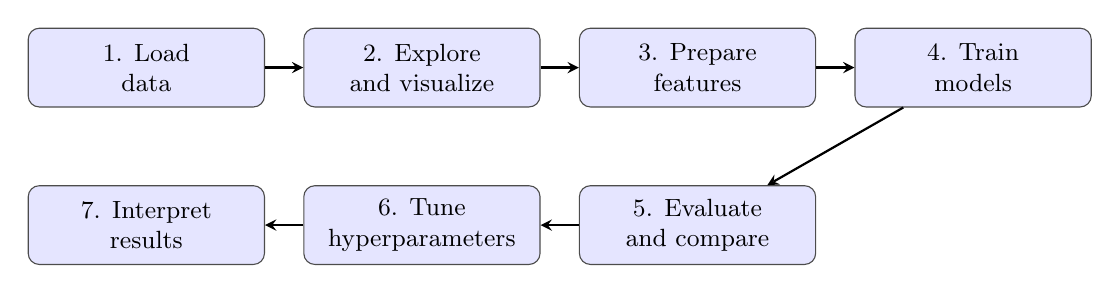
\begin{tikzpicture}[
    stepbox/.style={rectangle, draw=black!70, fill=blue!10, rounded corners, minimum width=3cm, minimum height=1cm, align=center, font=\small},
    arr/.style={->, thick, >=stealth}
]
\node[align=center,stepbox] (load) at (0, 0) {1. Load\\data};
\node[align=center,stepbox] (explore) at (3.5, 0) {2. Explore\\and visualize};
\node[align=center,stepbox] (prep) at (7, 0) {3. Prepare\\features};
\node[align=center,stepbox] (train) at (10.5, 0) {4. Train\\models};
\node[align=center,stepbox] (eval) at (7, -2) {5. Evaluate\\and compare};
\node[align=center,stepbox] (tune) at (3.5, -2) {6. Tune\\hyperparameters};
\node[align=center,stepbox] (interp) at (0, -2) {7. Interpret\\results};

\draw[arr] (load) -- (explore);
\draw[arr] (explore) -- (prep);
\draw[arr] (prep) -- (train);
\draw[arr] (train) -- (eval);
\draw[arr] (eval) -- (tune);
\draw[arr] (tune) -- (interp);
\end{tikzpicture}
\end{center}

\section{Exercises}

\begin{exercise}[$\star$]
Reproduce the Titanic project but add the \py{embarked} feature (one-hot encoded). Does it improve the model performance?
\end{exercise}

\begin{exercise}[$\star$]
On the California Housing dataset, train a simple linear regression using only \py{MedInc} as a feature. What $R^2$ do you obtain? Compare with the full model.
\end{exercise}

\begin{exercise}[$\star\star$]
For the Titanic project, create an ``age group'' feature (child: $<$12, teenager: 12--18, adult: 18--60, senior: $>$60). Does this engineered feature improve the random forest performance?
\end{exercise}

\begin{exercise}[$\star\star$]
On the California Housing dataset, compare linear regression, random forest, and gradient boosting (\py{GradientBoostingRegressor}) using 5-fold cross-validation. Which model gives the best $R^2$?
\end{exercise}

\begin{exercise}[$\star\star\star$]
Perform a complete end-to-end project on the \py{load_wine()} dataset: explore the data, handle preprocessing, compare at least three classifiers, tune the best model's hyperparameters, and present a detailed evaluation with confusion matrix and classification report.
\end{exercise}

\begin{exercise}[$\star\star\star$]
On the California Housing dataset, investigate whether geographic features can be improved by creating a ``distance to major cities'' feature (e.g., distance to San Francisco, Los Angeles, San Diego). Use the Haversine formula to compute distances from latitude and longitude. Does this feature engineering improve the model?
\end{exercise}

\begin{keyformulas}
\textbf{Summary of Chapter~\ref{ch:projets}}
\begin{itemize}
    \item \textbf{Complete workflow}: load, explore, prepare, train, evaluate, tune, interpret.
    \item \textbf{Feature engineering}: create meaningful features from raw data.
    \item \textbf{Missing values}: fill with median, mode, or use domain knowledge.
    \item \textbf{Model comparison}: always compare multiple models with cross-validation.
    \item \textbf{Hyperparameter tuning}: use \py{GridSearchCV} or \py{RandomizedSearchCV}.
    \item \textbf{Feature importance}: use \py{feature_importances_} to understand model decisions.
    \item \textbf{Classification metrics}: accuracy, precision, recall, F1-score.
    \item \textbf{Regression metrics}: MAE, RMSE, $R^2$.
\end{itemize}
\end{keyformulas}
